%%===========================================================%%
%%                                                           %%
%%                        BACKGROUNDS                        %%
%%                                                           %%
%%===========================================================%%

\chapter{Backgrounds}\label{chap:backgrounds}

\section{Sources of background}
\subsection{Non-exclusive background}\label{sec:nonExclBkgd}

The main background present in the final exclusive $\pi^{+}\pi^{-}/K^{+}K^{-}/p\bar{p}$ sample is the non-exclusive background. There are several classes of events which mimic topology of $h^{+}h^{-}$ CEP: two forward protons, two opposite sign central tracks and rapidity gaps. Below we list the most probable cases:
  \begin{itemize}
  \item Single physics processes:
  \begin{itemize}
  \item Central Diffraction (Fig.~\ref{fig:bkgdSources_cd}) - this process differs from CEP of $h^{+}h^{-}$ only by the number of particles produced in the mid-rapidity; protons originate from the same vertex as the central tracks, hence correlation of reconstructed vertex position from RPs and TPC is still observed.
  \end{itemize}
  \item Coincidences (pile-up):
  \begin{itemize}
  \item inelastic + elastic interaction (Fig.~\ref{fig:bkgdSources_mb_el}) - there may be overlap of protons from elastic scattering interaction and activity in the central detector from another (inelastic) interaction; it should be supressed by the rapidity gap veto in BBC-small (online) and BBC-large (offline); easy to identify through protons collinearity and lack of correlation of $z$-vertex from RPs and TPC.
  \end{itemize}\vspace*{-17pt}
  
  
  \hspace*{-7pt}$\left.
\begin{tabular}{p{.9\textwidth}}
  \begin{itemize}
  \item Single Diffraction + beam halo - there may be overlap of proton from SD on one side and beam halo proton on the opposite side, and activity in the central detector from diffractive state; it should be supressed by the rapidity gap vetos and (low) beam halo rate;
  \item  2$\times$beam halo + inelastic interaction.
  \end{itemize}
  \end{tabular}
\right\}_{\rotatebox{90}{~~~~negligibly low\hspace*{-25pt}}}$
  
 \end{itemize}

 These backgrounds are graphically presented in Fig.~\ref{fig:bkgdSources}.

%---------------------------
\begin{figure}[h]
\centering%
\parbox{0.315\textwidth}{%
  \centering%
  \begin{subfigure}[b]{0.9\linewidth}{
                \subcaptionbox{\label{fig:bkgdSources_cep}}{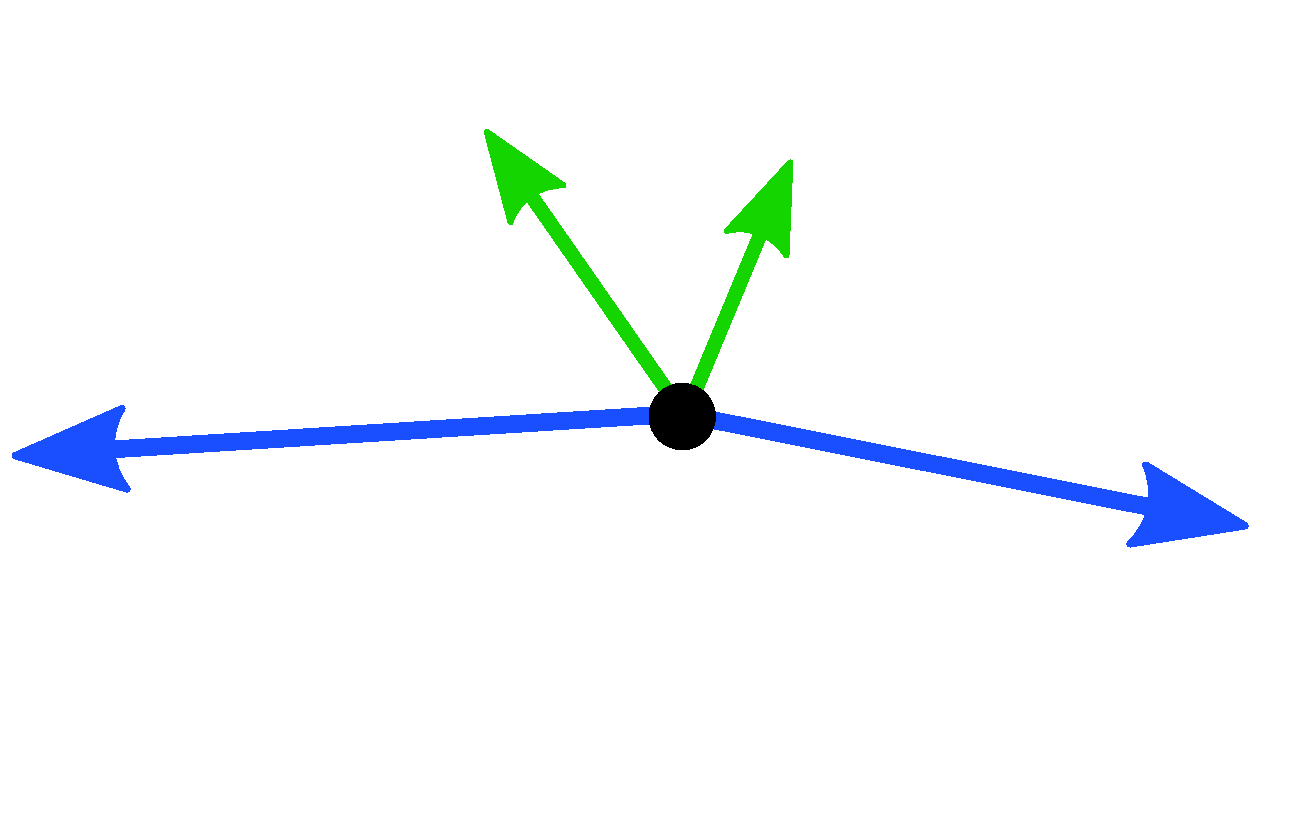
\includegraphics[width=\linewidth]{graphics/backgrounds/cep.pdf}}}
  \end{subfigure}
}%
\quad%
\parbox{0.315\textwidth}{%
  \centering%
  \begin{subfigure}[b]{0.9\linewidth}{
                \subcaptionbox{\label{fig:bkgdSources_cd}}{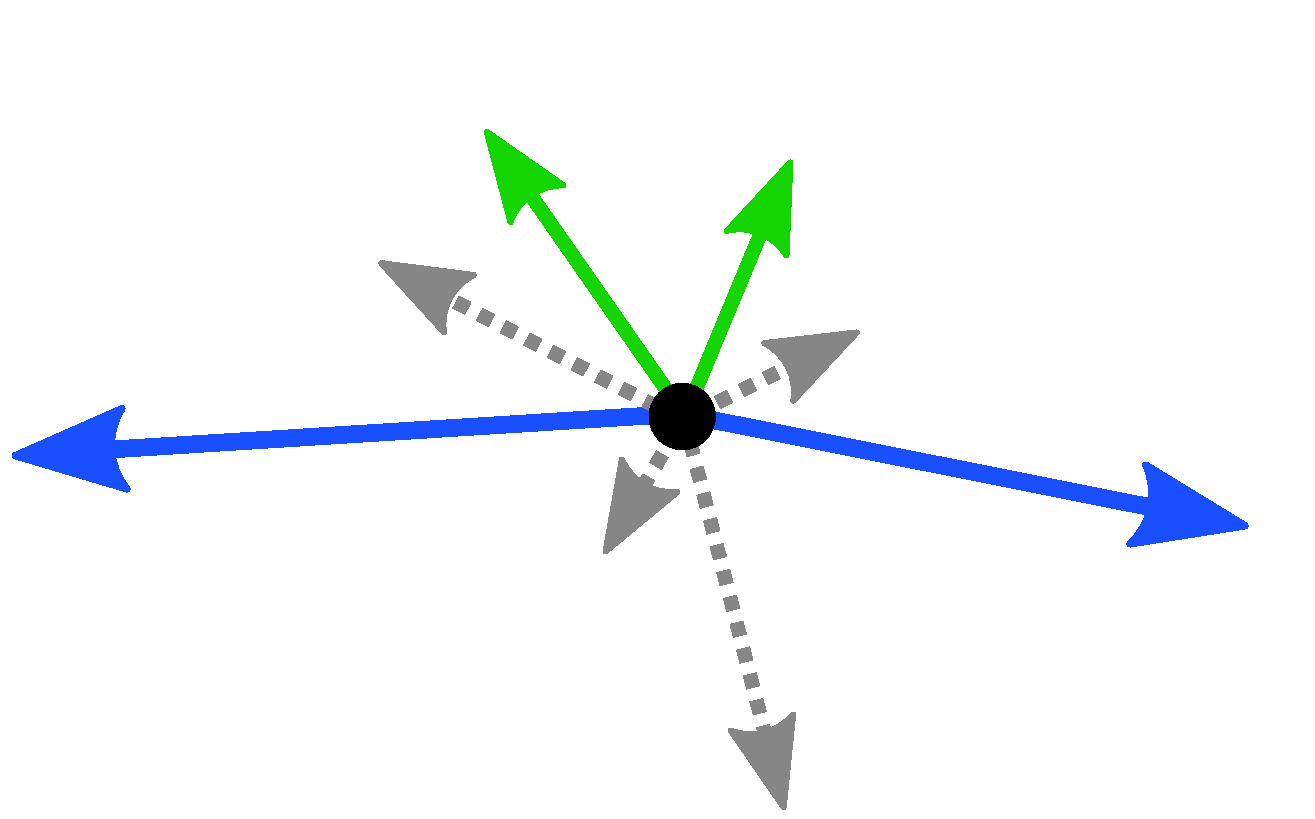
\includegraphics[width=\linewidth]{graphics/backgrounds/cd.pdf}}}
  \end{subfigure}
}%
\quad%
\parbox{0.315\textwidth}{%
  \centering%
  \begin{subfigure}[b]{0.9\linewidth}{
                \subcaptionbox{\label{fig:bkgdSources_mb_el}}{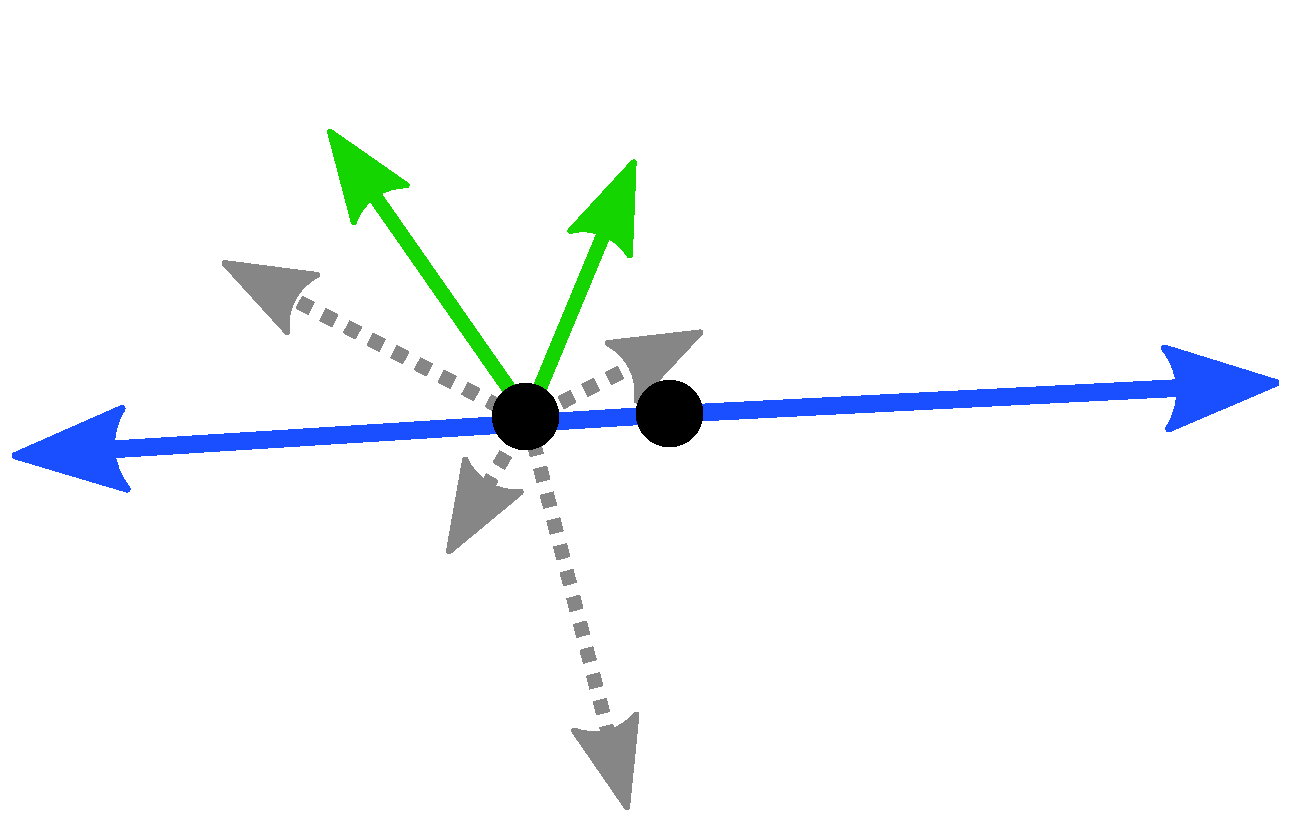
\includegraphics[width=\linewidth]{graphics/backgrounds/mb_el.pdf}}}
  \end{subfigure}
}%
\caption[Sketches of main processes with CEP event topology.]{Sketches of main processes exhibiting $h^{+}h^{-}$ CEP event topology: the exclusive $h^{+}h^{-}$ signal itself (\ref{fig:bkgdSources_cep}), central diffraction event with some particles not detected (\ref{fig:bkgdSources_cd}) and elastic proton-proton scattering event with pile-up inelastic interaction in the central region (\ref{fig:bkgdSources_mb_el}). Particles represented by arrows are: forward scattered protons (blue), detected mid-rapidity particles (green) and undetected particles (dashed gray). Black dots mark primary interaction vertices.}\label{fig:bkgdSources}
\end{figure}
%---------------------------
 
 

% %---------------------------
% \begin{figure}[h]
% \centering%
% 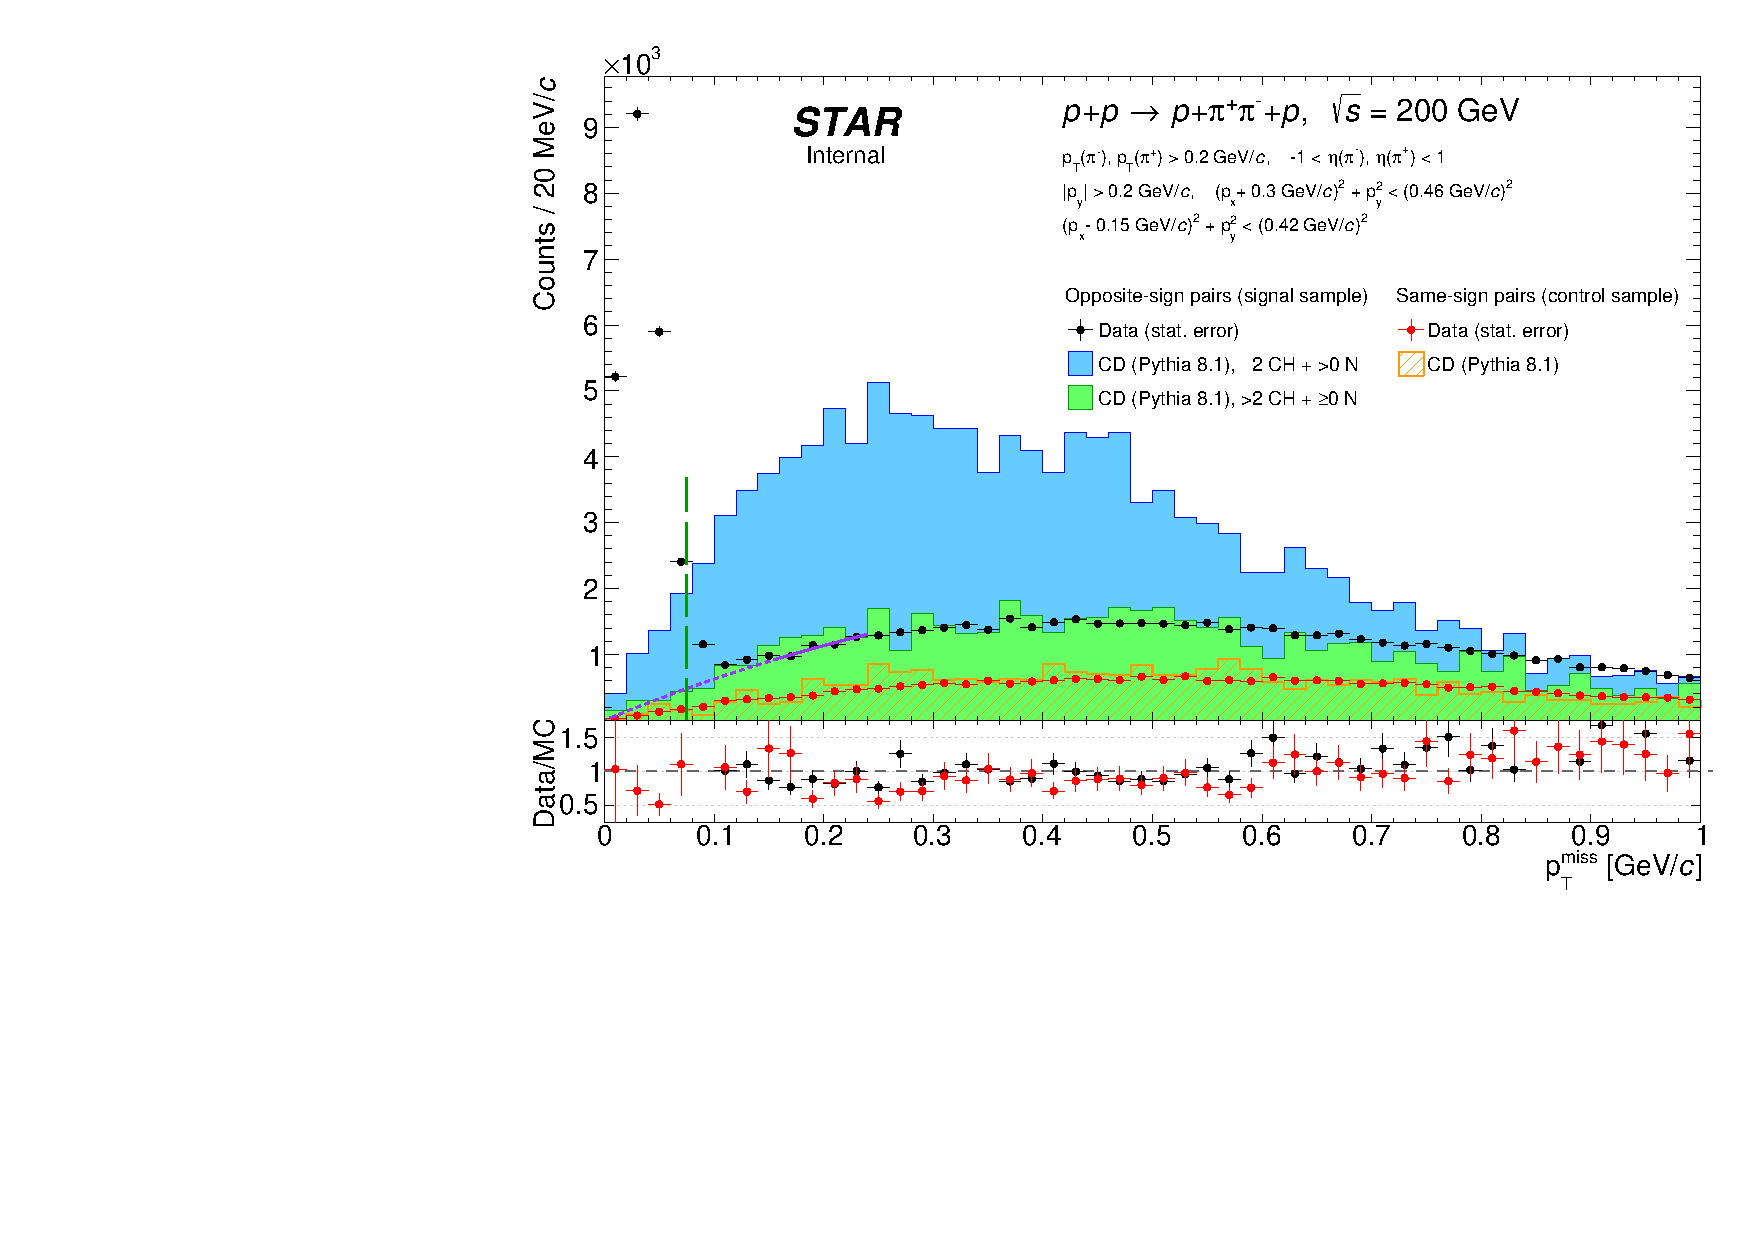
\includegraphics[width=0.65\linewidth,page=1]{graphics/backgrounds/Raw_MissingPtPid.pdf}%
% \caption{Missing pT.}\label{fig:missingPtBkgd}%
% \end{figure}
% %---------------------------
\newpage
\subsection{Exclusive background (particle misidentification)}\label{sec:exclBkgd}

Another source of background which is connected with finite particle identification power is the exclusive background from the particle species other than species under study.

%---------------------------
\begin{figure}[h]
\centering%
\parbox{0.4725\textwidth}{%
  \centering%
  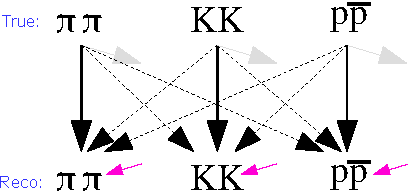
\includegraphics[width=\linewidth]{graphics/backgrounds/pid-crop2.pdf}\label{fig:misidentificationGraph}
}%
\quad%
\parbox{0.4725\textwidth}{%
    \caption[Graph illustrating the misidentification problem.]{Graph illustrating the misidentification problem - the origin of exclusive background in selected samples. Gray arrows represent event rejection due to failed PID selection (\ref{enum:CutPid}). Magenta arrows indicate non-exclusive backgrounds described in Sec.~\ref{sec:nonExclBkgd}. Solid black arrows represent successful identification, whereas dashed black lines show misidentification paths.}
}%

\end{figure}
%---------------------------


\begin{subequations}\label{eq:misidentificationEqs}
\begin{equation}
  N^{\pi\pi}_{R}~~=~~\begingroup\color{gray}\underbrace{\color{black}\epsilon^{\pi\pi}\cdot N^{\pi\pi}_{T}}_{\textrm{true pion pairs}}\endgroup~~ + ~~\begingroup\color{gray}\underbrace{\color{black}\lambda^{ KK\rightarrow \pi\pi}\cdot N^{KK}_{T}}_{\substack{\textrm{kaon pairs reconstructed} \\ \textrm{as pion pairs}}}\endgroup~~ + ~~\begingroup\color{gray}\underbrace{\color{black}\lambda^{p\bar{p} \rightarrow \pi\pi} \cdot N^{p\bar{p}}_{T}}_{\substack{\textrm{proton pairs reconstructed} \\ \textrm{as pion pairs}}}\endgroup~~ + ~~\textcolor{magenta}{N^{\pi\pi}_{bkgd}}
\end{equation}    
\begin{equation}
  N^{KK}_{R} ~= ~~\begingroup\color{gray}\underbrace{\color{black}\lambda^{ \pi\pi\rightarrow KK}\cdot N^{\pi\pi}_{T}}_{\substack{\textrm{pion pairs reconstructed} \\ \textrm{as kaon pairs}}}\endgroup~~ + ~~\begingroup\color{gray}\underbrace{\color{black}\epsilon^{KK}\cdot N^{KK}_{T}}_{\textrm{true kaon pairs}}\endgroup~~ + ~~\begingroup\color{gray}\underbrace{\color{black}\lambda^{p\bar{p} \rightarrow KK} \cdot N^{p\bar{p}}_{T}}_{\substack{\textrm{proton pairs reconstructed} \\ \textrm{as kaon pairs}}}\endgroup~~ + ~~\textcolor{magenta}{N^{KK}_{bkgd}}
\end{equation}
\begin{equation}\hspace*{-25pt}
  N^{p\bar{p}}_{R}~~~= ~~\begingroup\color{gray}\underbrace{\color{black}\lambda^{\pi\pi \rightarrow p\bar{p}} \cdot N^{\pi\pi}_{T}}_{\substack{\textrm{pion pairs reconstructed} \\ \textrm{as proton pairs}}}\endgroup~~ + ~~\begingroup\color{gray}\underbrace{\color{black}\lambda^{ KK\rightarrow p\bar{p}}\cdot N^{KK}_{T}}_{\substack{\textrm{kaon pairs reconstructed} \\ \textrm{as proton pairs}}}\endgroup~~ + ~~\begingroup\color{gray}\underbrace{\color{black}\epsilon^{p\bar{p}}\cdot N^{p\bar{p}}_{T}}_{\textrm{true proton pairs}}\endgroup~~ + ~~\textcolor{magenta}{N^{p\bar{p}}_{bkgd}}
\end{equation}
\end{subequations}

Eqs.~\eqref{eq:misidentificationEqs} can be written in the matrix form, as shown in Eq.~\eqref{eq:misidentificationMatrix}, from which it is straightforward to obtain final formula for unfolded number of events of given ID, Eq.~\eqref{eq:pidUnfoldingMatrix}:

\begin{tabulary}{\textwidth}{LCL}
\begin{equation}\label{eq:misidentificationMatrix}\hspace*{-15pt}
\Spvek{N^{\pi\pi}_{R}-\textcolor{magenta}{N^{\pi\pi}_{bkgd}};~;N^{KK}_{R}-\textcolor{magenta}{N^{KK}_{bkgd}};~;N^{p\bar{p}}_{R}-\textcolor{magenta}{N^{p\bar{p}}_{bkgd}}} =  \underbrace{\left[ \begin{array}{ccc}
\epsilon^{\pi\pi} & \lambda^{ KK\rightarrow \pi\pi} & \lambda^{p\bar{p} \rightarrow \pi\pi} \\
~ & ~ & ~\\
\lambda^{\pi\pi\rightarrow KK} & \epsilon^{KK} & \lambda^{ p\bar{p} \rightarrow KK}\\
~ & ~ & ~\\
\lambda^{\pi\pi\rightarrow p\bar{p}} & \lambda^{ KK\rightarrow p\bar{p}} & \epsilon^{p\bar{p}}
\end{array} \right]}_{\text{``mixing matrix''}~\Lambda}\Spvek{N^{\pi\pi}_{T};~;N^{KK}_{T};~;N^{p\bar{p}}_{T}}
\end{equation}&%
\vspace{40pt}$\rightarrow$\hspace{20pt}&
\begin{equation}\label{eq:pidUnfoldingMatrix}
\Spvek{N^{\pi\pi}_{T};~;N^{KK}_{T};~;N^{p\bar{p}}_{T}} = \Lambda^{-1}\Spvek{N^{\pi\pi}_{R}-\textcolor{magenta}{N^{\pi\pi}_{bkgd}};~;N^{KK}_{R}-\textcolor{magenta}{N^{KK}_{bkgd}};~;N^{p\bar{p}}_{R}-\textcolor{magenta}{N^{p\bar{p}}_{bkgd}}}
\end{equation}
\end{tabulary}

\section{Non-exclusive background determination}

Determination of non-exclusive background makes use of the missing transverse momentum which is distributed differently for the signal and for aforementioned background. High statistics of the data allows to apply a data-driven method. What is more, not only integrated over observables but even differentially as a function of these.

It has already been demonstrated in Sec.~\ref{subsec:ptMiss} that $p_{\text{T}}^{\text{miss}}$ from exclusive events is much narrower compared to background, visible as a peak near the axis origin. Additional feature of 
$p_{\text{T}}^{\text{miss}}$ - probability density approaching to zero with $p_{\text{T}}^{\text{miss}}$ moving towards the axis origin, enables performing a polynomial fit to $p_{\text{T}}^{\text{miss}}$ distribution in the background-dominated range and extrapolation of this polynomial down to  $p_{\text{T}}^{\text{miss}} = 0$ under the peak of CEP signal. The procedure used to determine non-exclusive background content in the signal region is described below.

%\begin{enumerate}
% \item 2-dimensional histograms of quantities of interest $q$ (probe $\eta$, probe $p_{T}$, $z_{\text{vtx}}$) vs. $p_{T}^{\text{miss}}$ were filled, separately for all probes and only for probes matched with TOF. Each probe (each entry to the histogram) was associated with the weight $w$ taking into account the trigger efficiency and vertexing efficiency, as given in Eq.~\eqref{eq:tagAndProbeWeight} and explained later in the text.\\[-20pt]%
%%
%\item In each bin of quantity of interest $q$ (as a function of which the efficiency was to be determined) the distribution of $p_{T}^{\text{miss}}$ was fitted in the signal-free region with the function describing background shape. The background function was extrapolated to $p_{T}^{\text{miss}}=0$. The signal yield in given bin of $q$ was calculated as the integral of the histogram with subtracted integral of the background function, both in the range $p_{T}^{\text{miss}}<75$~MeV.
%\end{enumerate}

\section{Normalization of signal and background models}\label{sec:bkgdSignalNorm}

